\section{Experiments}
% \begin{figure}
%   \centering
%   \begin{subfigure}[b]{0.48\linewidth}
%     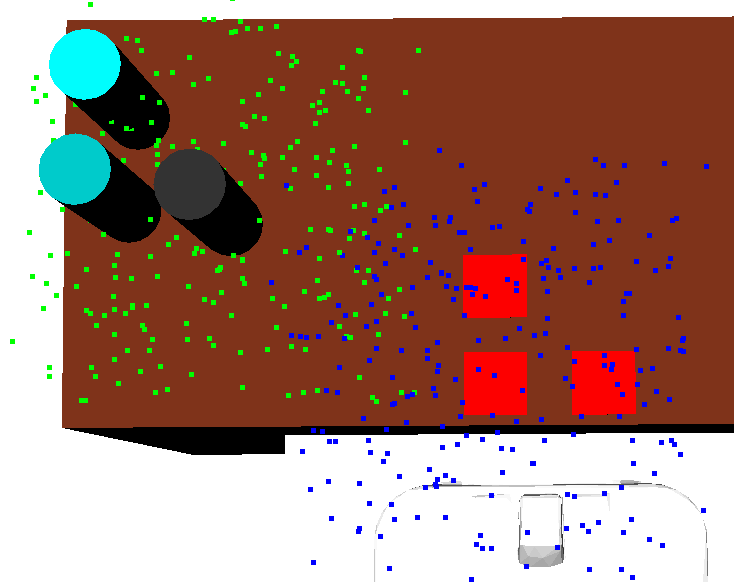
\includegraphics[width=\textwidth]{images/learns.png}
%     \caption{Initial distribution}
%   \end{subfigure}
%   \begin{subfigure}[b]{0.48\linewidth}
%     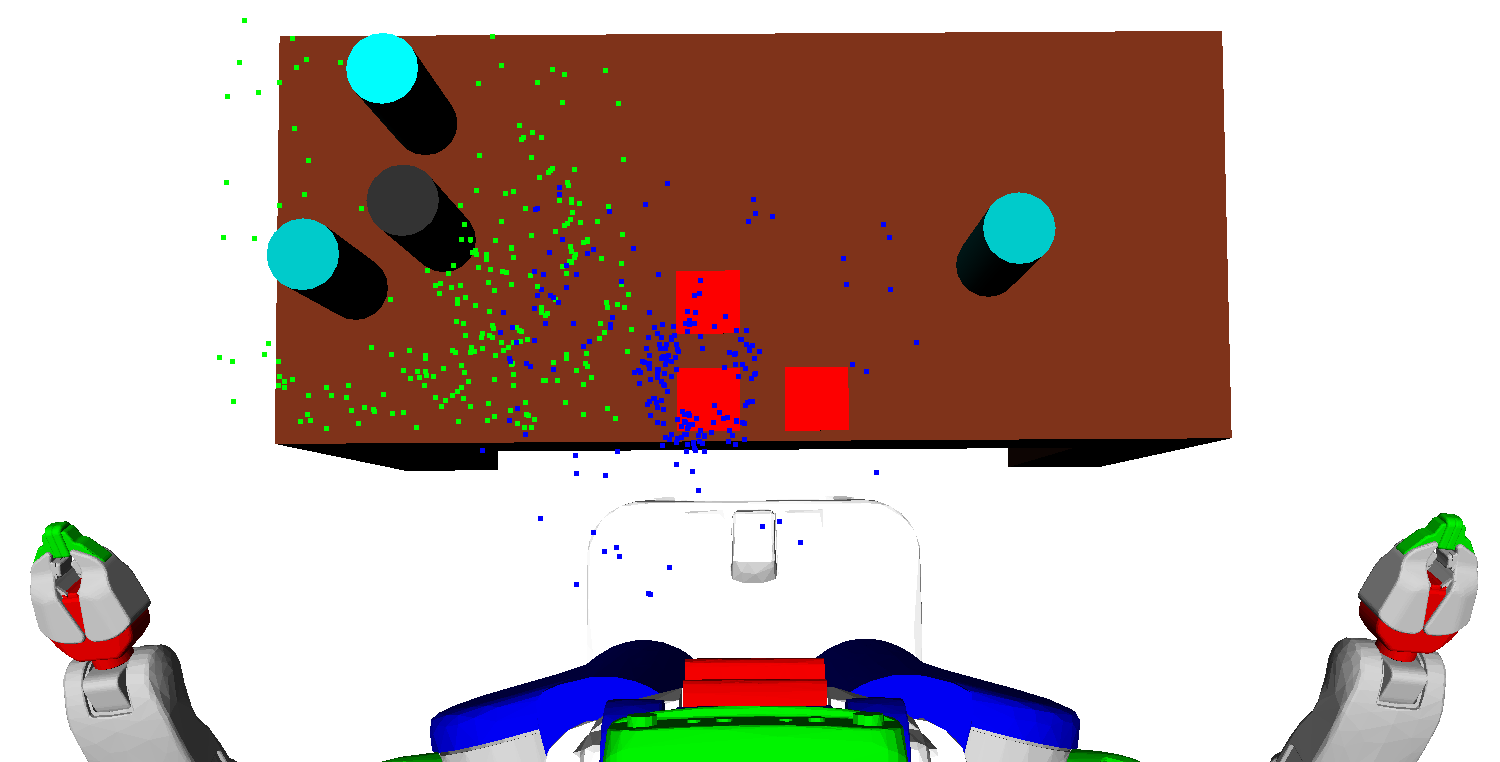
\includegraphics[width=\textwidth]{images/learn10.png}
%     \caption{After 10 iterations.}
%   \end{subfigure}
%   \begin{subfigure}[b]{0.48\linewidth}
%     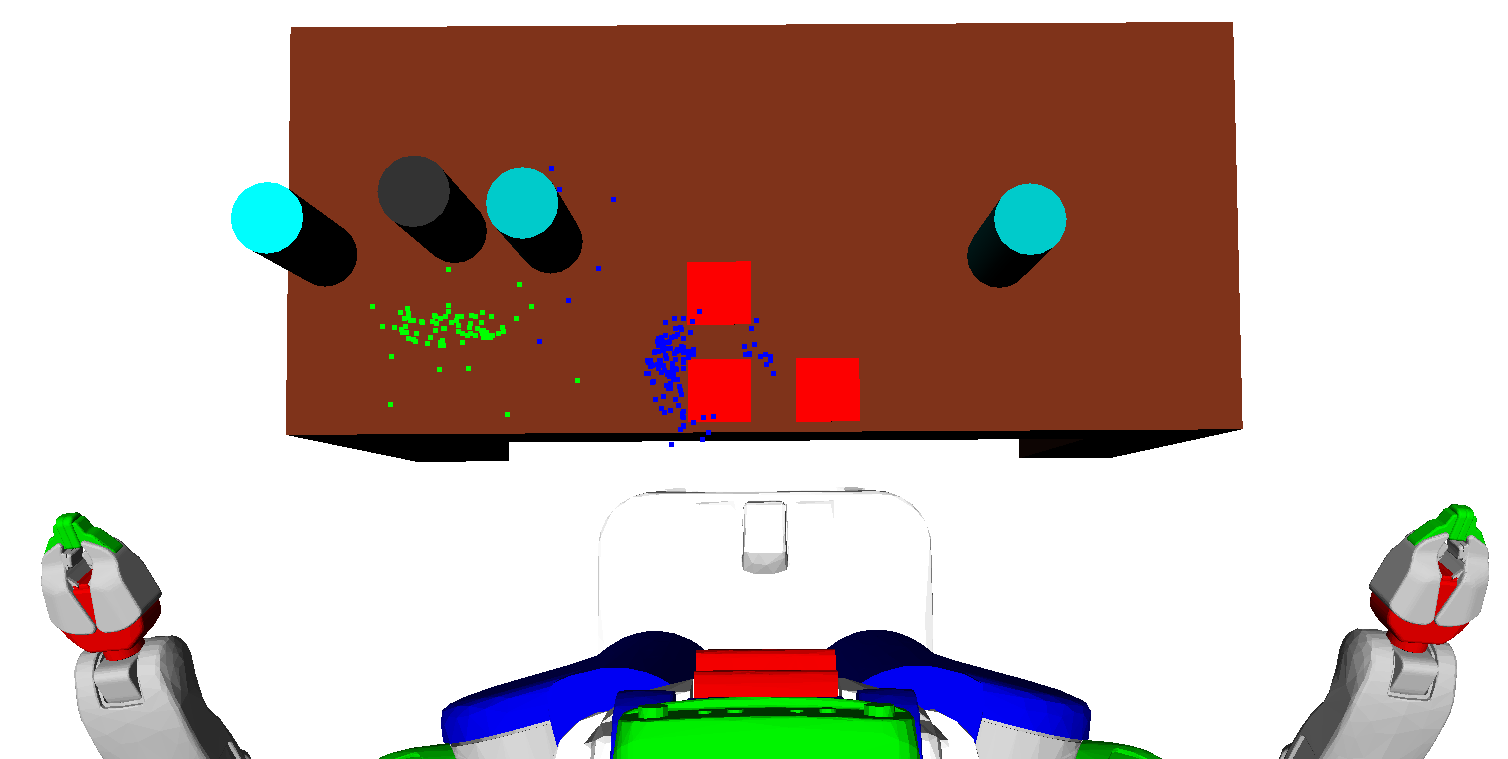
\includegraphics[width=\textwidth]{images/learn15.png}
%     \caption{After 15 iterations.}
%   \end{subfigure}
%   \begin{subfigure}[b]{0.48\linewidth}
%     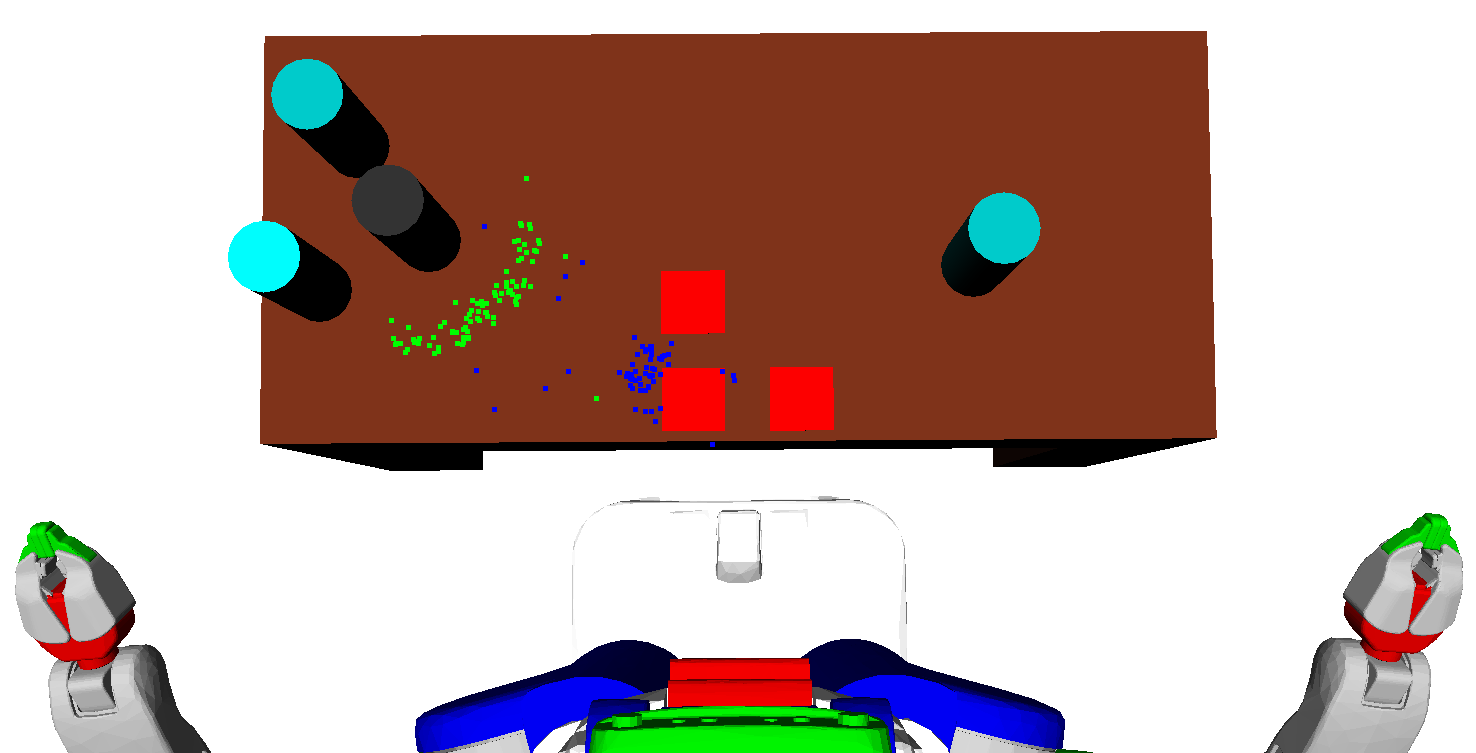
\includegraphics[width=\textwidth]{images/learn20.png}
%     \caption{Final distribution.}
%   \end{subfigure}
%   \caption{Learned left arm grasp (green) and putdown (blue) distributions used to
% pick up the black can and place it on the central red square, after different training iterations.
% An iteration refers to a single run of randomized refinement,
% which terminates after $L$ calls to the \texttt{resample} routine. The
% initial distributions are uniform because we initialize weights to $\vec{\mathbf{0}}$.
% The final distributions are after 20 iterations. The convergence and robustness of
% the distributions demonstrate the soundness of our approach.}
%   \label{fig:training}
% \end{figure}

% \begin{figure}
%   \centering
%   \begin{subfigure}[b]{0.3\linewidth}
%     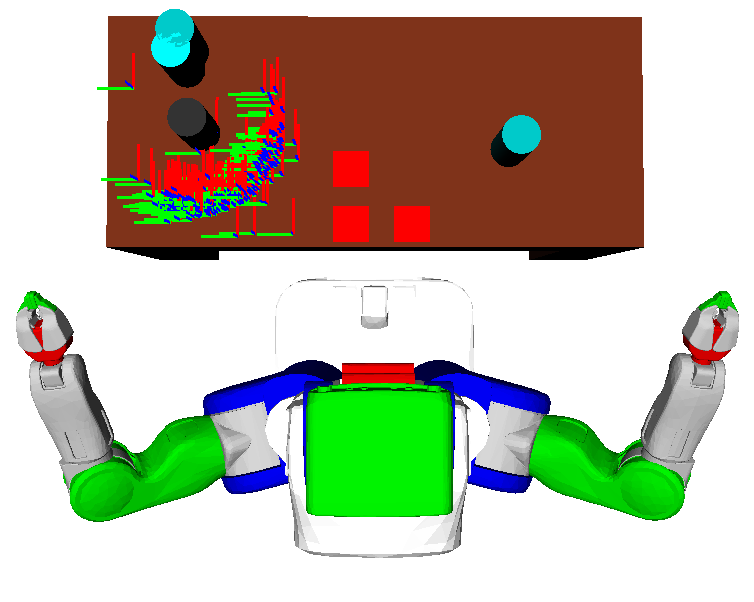
\includegraphics[width=\textwidth]{images/finalgraspnoobstr.png}
%     \caption{}
%   \end{subfigure}
%   \begin{subfigure}[b]{0.3\linewidth}
%     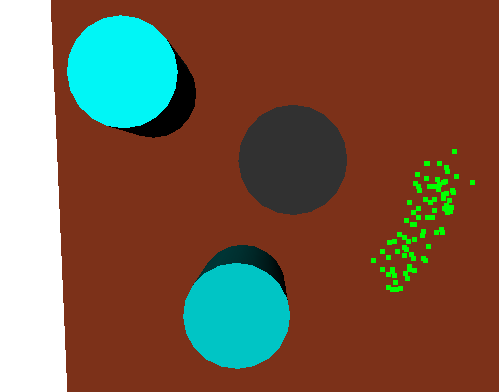
\includegraphics[width=\textwidth]{images/finalgraspobstr.png}
%     \caption{}
%   \end{subfigure}
%   \begin{subfigure}[b]{0.3\linewidth}
%     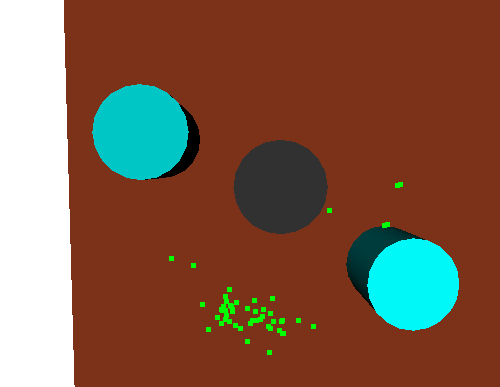
\includegraphics[width=\textwidth]{images/finalgraspobstr2.png}
%     \caption{}
%   \end{subfigure}
%   \caption{The learned grasp pose distribution
% is shown with different obstruction layouts. The system learns to
% avoid obstructions while providing a good set of grasping poses.}
%   \label{fig:obstr}
% \end{figure}

\begin{table}
  \centering
  \vspace{8pt}
  \tabcolsep=0.11cm{
  \begin{tabular}{ccccc}
    \toprule[1.5pt]
      \textbf{\# Objects} & \textbf{System} & \textbf{\% Solved (SD)} & \textbf{Avg MP Time (s)} & \textbf{Avg \# MP Calls}\\
    \midrule[2pt]
      2 (dinner) & B & TODO (X) & 0 & 0\\
    \midrule
      2 (dinner) & L & TODO (X) & 0 & 0\\
    \midrule[1.5pt]
      4 (dinner) & B & TODO (X) & 0 & 0\\
    \midrule
      4 (dinner) & L & TODO (X) & 0 & 0\\
    \midrule[1.5pt]
      25 (cans) & B & 74 (0) & 15.1 & 19.0\\
    \midrule
      25 (cans) & L & 84 (5.1) & 12.4 & 12.6\\
    \midrule
      25 (cans) & F & 92 (5.8) & 10.7 & 12.0\\
    \midrule[1.5pt]
      30 (cans) & B & 36 (0) & 48.2 & 35.4\\
    \midrule
      30 (cans) & L & 69 (8.0) & 21.9 & 19.0\\
    \midrule
      30 (cans) & F & 77 (6.5) & 23.1 & 21.8\\
    \bottomrule[1.5pt]
  \end{tabular}}
  \caption{Percent solved and standard deviation, along with time spent motion planning and number of calls to the motion
planner for the baseline system (B), our system with only learned refinement policies (no graph search heuristics) (L),
and our full system (F). Results using our system are averaged across 10 different sets of weights. Time limit: 300s.}
  \label{table:results}
\end{table}

Our experiments are conducted in Python 2.7 using the OpenRave simulator~\cite{Diankov_2008_6117} with a PR2 robot.
The motion planner we use is trajopt~\cite{schulman2013finding}, and the task planner is Fast-Forward~\cite{FF}.
The experiments were carried out in series on an Intel Core i7-4790K machine with 16GB RAM.

We evaluate our approach in two distinct domains: cans distributed on a table (the \emph{can domain})
and setting up bowls for dinner (the \emph{dinner domain}).
We compare performance with that of the hand-coded sampling distributions and default plan refinement graph search
strategy used in Srivastava et al.~\cite{srivastava2014combined}. In both domains, plan refinement samples
are drawn from continuous distributions trained using the described algorithms. For the can domain, we
show results both with and without our trained heuristics for searching the plan refinement graph. However,
for the dinner domain, objects in the environment are never obstructed by others, so the default search policy
of picking the deepest node in the graph to refine is already optimal.

We use the reward function described earlier. Our weight
vectors are initialized to $\vec{\mathbf{0}}$ for all parameter types -- this
initialization represents a uniform distribution across the limits of the geometric search space.
We use 24 features. 9 binary features encode the bucketed distance between the sample
and target. 9 binary features encode the bucketed sample height. 3 features
describe the number of other objects within discs of radius 7, 10, and 15 centimeters around the
sample. 3 binary features describe the angle made between the vector from the
robot to the target and the vector from the sample to the target: whether the angle is less than
$\pi/3$, $\pi/2$, and $3\pi/4$.

For the can domain, the goal across all experiments is for the robot to pick up a particular object with its
left gripper. We disabled the right gripper, so any obstructions to the target object must be picked up and
placed elsewhere on the table. This domain has 4 types of continuous parameters: base poses, object grasp
poses, object putdown poses, and object putdown locations onto the table. The range of allowable values for
grasp and putdown poses is a cube of side length 30 centimeters around
the target object or putdown location. For base poses, the range is a
square of side length 1 meter around the object or location which the robot is approaching. For putdown locations,
the range is defined by the edges of the table.

Initial experimentation revealed that training jointly for all these continuous
parameter types was infeasible due to a dearth of valid plan refinements being produced, so we decided to
incorporate curriculum learning. Thus, we train $N = 10$ iterations of plans involving just base motion and grasping,
then $N = 20$ iterations of base motion, grasping, and putdown at a predefined location, then $N = 30$ iterations of
the full set of parameter types, including a varying putdown location. We fixed $L = 100$ and $\epsilon = 20$.

For the experiments which only use the trained plan refinement policies (no learned heuristics for searching the plan
refinement graph), we trained 10 different sets of weights using the described curriculum learning system, varying
only the random number generator's initial seed. Then, for the experiments which also search the plan refinement graph
intelligently, we employed an improved training methodology to reduce variation due to seeding. We trained 30 different
sets of weights, and for every group of 3 sets, we picked the best one based on performance in a validation set and discarded
the other two. To test performance, we randomly generated 50 environments for both 25 cans and 30 cans on the table,
and measured success rate, motion planning time, and number of motion planner calls for the baseline system and each
trained set of weights.

For the dinner domain, we run two sets of experiments, in which the robot must move 2 and 4
bowls from their initial location on one table to target locations on the other. We assign a cost to
base motion in the environment, so the robot is encouraged to use the provided tray, onto which bowls can be stacked.
This domain has 5 types of continuous parameters: base poses, object grasp poses, object putdown poses, tray pickup
poses, and tray putdown poses. Our curriculum learning system first trains the tray pickup and putdown poses for
$N = 20$ iterations, then the object grasp and putdown poses for $N = 20$ iterations. We fixed $L = 100$ and $\epsilon = 10$.
We trained 10 different sets of weights (varying only the seed) and tested performance across 50 randomly generated
environments for each number of objects.

Table \ref{table:results} summarizes our quantitative results, which demonstrate
comparable performance to the baseline system for the dinner domain, and significant improvements for
the can domain. The reason performance does not greatly improve for the dinner domain is that the
hand-coded discretizations of the sample space are very good in this environment. For example, the optimal
robot base pose from which to pick up the tray is directly in front of it, which is quickly found through
the baseline system's discretization for the tray pickup pose parameter.